\section{正态分布}

~

{\bf 正态分布},也称{\bf 高斯分布},记作$N\left( \mu ,\sigma ^2 \right) $,类似泊松分布,描述一个范围内的分布情况:
\[
f\left( x \right) =\frac{1}{\sqrt{2\pi}\sigma}e^{-\frac{\left( x-\mu \right) ^2}{2\sigma ^2}},\qquad \mu \in \mathbb{R} ,\sigma >0
\]
其中:
\begin{itemize}
    \item $\mu $:数学期望,规定了中心点的横坐标,$f\left( x \right) $以$x=\mu $为对称,并在$x=\mu $取得最大值$\frac{1}{\sqrt{2\pi}\sigma}$;
    \item $\sigma $:标准差,一方面规定了$f\left( x \right) $的两个拐点$\mu \pm \sigma $,另一方面也规定了平坦度,$\sigma $越大,曲线越平坦。
\end{itemize}
特别地,当$\mu =0,\sigma =1$时,称为{\bf 标准正态分布},记作$N\left( 0,1 \right) $,此时密度函数和分布函数通常记为$\varphi \left( x \right) ,\varPhi \left( x \right) $,有:
\[
\varphi \left( x \right) =\frac{1}{\sqrt{2\pi}}e^{-\frac{x^2}{2}}\qquad \varPhi \left( x \right) =\int_{-\infty}^x{\varphi \left( t \right) \cdot dt}
\]
根据密度函数的偶函数定理,有性质:
\begin{align*}
&\varPhi \left( x \right) +\varPhi \left( -x \right) =1 \\
&\varPhi \left( 0 \right) =0.5
\end{align*}

\begin{figure}[h]
\centering
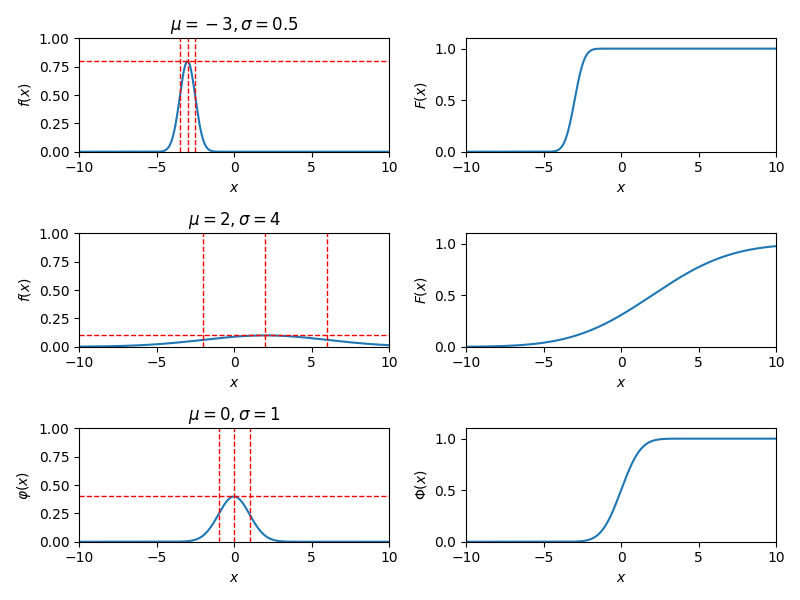
\includegraphics[height=7.5cm]{7.5-1.png}
\end{figure}

\begin{tcolorbox}
正态分布常用于描述身高、体重、成绩、元器件指标等的离散程度。
\end{tcolorbox}

\begin{theorem}
若$X\sim N\left( \mu ,\sigma ^2 \right) $,则有:
\[
P\left\{ a<X\leqslant b \right\} =\varPhi \left( \frac{b-\mu}{\sigma} \right) -\varPhi \left( \frac{a-\mu}{\sigma} \right)
\]
\end{theorem}

可用积分变量替换进行证明,略。该定理使得我们可以用标准分布计算任何正态分布。

\begin{theorem}
设$X_1\sim N\left( \mu _1,{\sigma _1}^2 \right) ,X_2\sim N\left( \mu _2,{\sigma _2}^2 \right) $ ,则$Y=X_1+X_2$也服从正态分布,且有:
\begin{align*}
&Y\sim N\left( \mu _1+\mu _2,{\sigma _1}^2+{\sigma _2}^2 \right) \\
&f\left( y \right) =\frac{1}{\sqrt{2\pi \left( {\sigma _1}^2+{\sigma _2}^2 \right)}}e^{-\frac{\left[ y-\left( \mu _1+\mu _2 \right) \right] ^2}{2\left( {\sigma _1}^2+{\sigma _2}^2 \right)}}
\end{align*}
反之,若正态分布$Y$能表示成两个变量的和$Y=X_1+X_2$,则$X_1,X_2$也必然是正态分布,这点被称为正态分布的{\bf 再生性}。
\end{theorem}

\begin{tcolorbox}
正态分布有很多特别的表现。一方面,若足够多的独立分布叠加,则总体可看成正态分布;另一方面,在相同方差的情况下,正态分布具有最大的不确定性。所以正态分布不但非常常见,而且也是优先考虑使用的模型。
\end{tcolorbox}

%============================================================
\subsection{习题}

\begin{example}[综合运用4,难度:$\star $]
袋装食盐标准质量为400g,规定误差的绝对值不超过4g就认为合格。假设误差服从正态分布,随机抽取100袋食盐,误差的样本均值为0,样本方差为4。请你估计这批袋装食盐的合格率。
\end{example}

解:

设每袋食盐的质量为随机变量$X$,则$X~N\left( 0,4^2 \right) $,误差的绝对值不超过4g就认为合格,于是食盐质量在$\pm 4$内的概率为:
\[
P\left\{ X\in \left[ -4,4 \right] \right\} =P\left\{ X\in \left[ -\sigma ,\sigma \right] \right\} =0.6827
\]
后略。

\begin{tcolorbox}
本题考察正态分布的概念,没有难度。
\end{tcolorbox}




